\caulc
\begin{ex}%[1D6N3-2]%[TDMZZ25]%%[Lê Phúc]
	Tập xác định của hàm số $y=(2+\cos x)^{\tfrac{1}{3}}$ là
	\choice
	{$(-2;+\infty)$}
	{\True $\mathbb{R}$}
	{$(0;+\infty)$}
	{$(1;+\infty)$}
	\loigiai{
		Vì $-1\le\cos x\le 1$ nên $1\le 2+\cos x\le 3$, suy ra $2+\cos x>0$ với mọi $x\in\mathbb{R}$.\\
		Vậy tập xác định của hàm số là $\mathscr{D}=\mathbb{R}$.
	}
\end{ex}

\begin{ex}%[1D3H2-3]%[TDMZZ25]%%[Lê Phúc]
	Giá trị $\lim\limits_{x\to-\infty}\dfrac{\sqrt{x^4-x+1}}{x^3-2x}$ bằng
	\choice
	{$1$}
	{$-1$}
	{\True $0$}
	{$+\infty$}
	\loigiai{
		Ta có $\sqrt{x^4-x+1}=x^2\sqrt{1-\dfrac{1}{x^3}+\dfrac{1}{x^4}}$ và $x^3-2x=x^3\left(1-\dfrac{2}{x^2}\right)$.\\
		Suy ra
		\[\lim\limits_{x\to-\infty}\dfrac{\sqrt{x^4-x+1}}{x^3-2x}=\lim\limits_{x\to-\infty}\dfrac{x^2\sqrt{1-\dfrac{1}{x^3}+\dfrac{1}{x^4}}}{x^3\left(1-\dfrac{2}{x^2}\right)}=\lim\limits_{x\to-\infty}\dfrac{1}{x}\cdot\dfrac{\sqrt{1-\dfrac{1}{x^3}+\dfrac{1}{x^4}}}{1-\dfrac{2}{x^2}}=0.\]
	}
\end{ex}

\begin{ex}%[1D6N2-2]%[TDMZZ25]%%[Lê Phúc]
	Cho hai số thực dương $a$, $b$. Hệ thức đúng là
	\choice
	{$\log\left(a^6b\right)=6\log a\log b$}
	{$\log\left(a^6b\right)=\log a+6\log b$}
	{\True $\log\left(a^6b\right)=6\log a+\log b$}
	{$\log\left(a^6b\right)=6\log a-\log b$}
	\loigiai{
		Ta có
		\[\log\left(a^6b\right)=\log a^6+\log b=6\log a+\log b.\]
	}
\end{ex}

\begin{ex}%[2D1N1-1]%[TDMZZ25]%%[Lê Phúc]
	Hàm số $f(x)=x^3-3x$ đồng biến trên khoảng
	\choice
	{\True $(-\infty;-1)$}
	{$(-\infty;1)$}
	{$(-1;+\infty)$}
	{$(-1;1)$}
	\loigiai{
		Tập xác định $\mathscr{D}=\mathbb{R}$.\\
		Ta có $f'(x)=3x^2-3$, $f'(x)=0\Leftrightarrow\hoac{&x=-1\\&x=1.}$\\
		Bảng biến thiên
		\begin{center}
			
\begin{tikzpicture}
				\tkzTabInit[nocadre=false,lgt=1.2,espcl=3,deltacl=0.5]
				{$x$/0.7,$f'(x)$/0.7,$f(x)$/2.1}
				{$-\infty$,$-1$,$1$,$+\infty$}
				\tkzTabLine{,+,0,-,0,+,}
				\tkzTabVar{-/$-\infty$,+/$2$,-/$-2$,+/$+\infty$}
			\end{tikzpicture}
		\end{center}
		Dựa vào bảng biến thiên, hàm số đồng biến trên khoảng $(-\infty;-1)$ và $(1;+\infty)$.
	}
\end{ex}

\begin{ex}%[2D4N1-2]%[TDMZZ25]%%[Lê Phúc]
	Họ nguyên hàm của hàm số $f(x)=3x^2-2x$ là
	\choice
	{$x^3-2x^2+C$}
	{$3x^3-x^2+C$}
	{\True $x^3-x^2+C$}
	{$x^3-2x+C$}
	\loigiai{
		Ta có $\displaystyle\int\left(3x^2-2x\right)\mathrm{\,d}x=x^3-x^2+C$.
	}
\end{ex}

\begin{ex}%[2H5N2-2]%[TDMZZ25]%[Lê Phúc]
	Trong không gian với hệ trục tọa độ $Oxyz$, cho đường thẳng $d\colon\dfrac{x+2}{2}=\dfrac{y-3}{-1}=\dfrac{z}{3}$. Một vectơ chỉ phương của đường thẳng $d$ là
	\choice
	{\True $\overrightarrow{u}_1=(2;-1;3)$}
	{$\overrightarrow{u}_2=(2;1;3)$}
	{$\overrightarrow{u}_3=(2;-3;0)$}
	{$\overrightarrow{u}_4=(3;1;-2)$}
	\loigiai{
		Đường thẳng $d\colon\dfrac{x+2}{2}=\dfrac{y-3}{-1}=\dfrac{z}{3}$ có một vectơ chỉ phương là $\overrightarrow{u}=(2;-1;3)$.
	}
\end{ex}

\begin{ex}%[2D4N3-1]%[TDMZZ25]%[Lê Phúc]
	Diện tích hình phẳng giới hạn bởi các đường $f(x)=x^2-3x$, $Ox$, $x=1$, $x=4$ bằng
	\choice
	{$2$}
	{$\dfrac{3}{2}$}
	{$\dfrac{22}{3}$}
	{\True $\dfrac{31}{6}$}
	\loigiai{
		Diện tích hình phẳng cần tìm bằng
		\[S=\displaystyle\int\limits_{1}^{4}\left|x^2-3x\right|\mathrm{\,d}x=\dfrac{31}{6}.\]}
\end{ex}

\begin{ex}%[2H2H1-2]%[TDMZZ25]%[Lê Phúc]
	Cho hình lăng trụ đứng $ABC. A'B'C'$. Đáp án cho nhận xét \textbf{sai} là
	\choice
	{$\left(\overrightarrow{AB}+\overrightarrow{B'C'}+\overrightarrow{C'A'}\right)\overrightarrow{BC}=0$}
	{$\left(\overrightarrow{AB}+\overrightarrow{BC}+\overrightarrow{C'A'}\right)\overrightarrow{BC}=0$}
	{$\left(\overrightarrow{AB'}+\overrightarrow{B'C'}+\overrightarrow{C'A'}\right)\overrightarrow{BC}=0$}
	{\True $\left(\overrightarrow{AB}+\overrightarrow{BC'}+\overrightarrow{C'B'}\right)\overrightarrow{BC}=0$}
	\loigiai{
		\immini{Ta có $\overrightarrow{B'C'}=\overrightarrow{BC}$ và $\overrightarrow{C'A'}=\overrightarrow{CA}$.\\
			Suy ra
			\begin{itemize}
				\item $\left(\overrightarrow{AB}+\overrightarrow{B'C'}+\overrightarrow{C'A'}\right)\overrightarrow{BC}=\left(\overrightarrow{AB}+\overrightarrow{BC}+\overrightarrow{CA}\right)\overrightarrow{BC}=\overrightarrow{0}\cdot\overrightarrow{BC}=0$.
				\item $\left(\overrightarrow{AB}+\overrightarrow{BC}+\overrightarrow{C'A'}\right)\overrightarrow{BC}=\left(\overrightarrow{AB}+\overrightarrow{BC}+\overrightarrow{CA}\right)\overrightarrow{BC}=\overrightarrow{0}\cdot\overrightarrow{BC}=0$.
				\item $\left(\overrightarrow{AB'}+\overrightarrow{B'C'}+\overrightarrow{C'A'}\right)\overrightarrow{BC}=\left(\overrightarrow{AC'}+\overrightarrow{C'A'}\right)\overrightarrow{BC}=\overrightarrow{AA'}\cdot\overrightarrow{BC}=0$.
			\end{itemize}
			Vậy khẳng định sai là $\left(\overrightarrow{AB}+\overrightarrow{BC'}+\overrightarrow{C'B'}\right)\overrightarrow{BC}=\overrightarrow{AB'}\cdot \overrightarrow{BC}=0$.}
		{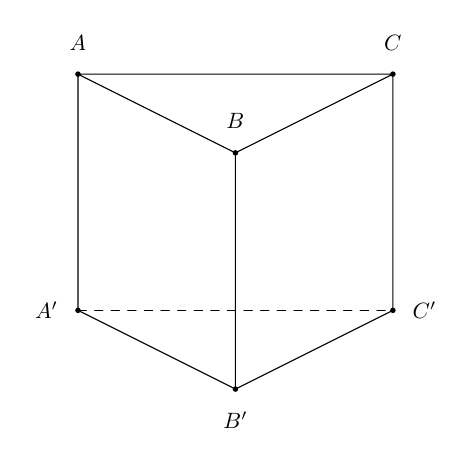
\begin{tikzpicture}[scale=1, line join=round, line cap=round, >=stealth]
				\tikzset{every node/.style={scale=0.8}}  			
				\coordinate (A') at (0,0);
				\coordinate (B') at (2,-1);
				\coordinate (C') at (4,0);
				\coordinate (A) at (0,3);
				\coordinate (B) at (2,2);
				\coordinate (C) at (4,3);
				\draw[dashed] (A')--(C');
				\draw (A')--(B')--(C') (A)--(B)--(C)--cycle (A)--(A') (B)--(B') (C)--(C');
				\foreach \i/\g in {A/90,B/90,C/90,A'/180,B'/-90,C'/0}
				\fill[black] (\i) circle(1pt)+(\g:4mm)node[scale=1]{$\i$};			
		\end{tikzpicture}}
	}
\end{ex}

\begin{ex}%[1D5H1-3]%[TDMZZ25]%[Lê Phúc]
	Cho một mẫu số liệu ghép nhóm $M$ có $7$ nhóm, mỗi nhóm đều có tần số bằng nhau. Số trung bình cộng của nhóm bằng phần tử đại diện của nhóm thứ
	\choice
	{$1$}
	{$5$}
	{\True $4$}
	{$3$}
	\loigiai{
		Gọi $x_1$, $x_2$, $\ldots$, $x_7$ lần lượt là giá trị đại diện của $7$ nhóm.\\
		Do tần số của mỗi nhóm đều bằng nhau và bằng $n$ nên tổng số phần tử mẫu là $7n$.\\
		Số trung bình cộng của mẫu số liệu ghép nhóm là
		\[\overline{x}=\dfrac{n \cdot x_1 + n \cdot x_2 + \dots + n \cdot x_7}{7n} = \dfrac{x_1 + x_2 + \dots + x_7}{7}.\]
		Vì các nhóm ghép nối tiếp liên tục và có độ rộng bằng nhau nên các giá trị đại diện $x_1$, $x_2$, $\ldots$, $x_7$ lập thành một cấp số cộng.\\
		Do đó, trung bình cộng của cấp số cộng có $7$ số hạng chính bằng số hạng đứng chính giữa, tức là số hạng thứ $4$ ($x_4$).
	}
\end{ex}

\begin{ex}%[2H5H1-3]%[TDMZZ25]%[Lê Phúc]
	Trong không gian $Oxyz$, cho mặt phẳng $(P)\colon2x-y-2z-1=0$. Mặt phẳng $(Q)$ đi qua gốc $O$ và song song với $(P)$ là
	\choice
	{$2x+y-2z=0$}
	{\True $2x-y-2z=0$}
	{$2x-y-2z+1=0$}
	{$2x+2y-z=0$}
	\loigiai{
		Mặt phẳng $(Q)$ song song với mặt phẳng $(P)\colon2x-y-2z-1=0$ nên
		\[(Q)\colon2x-y-2z+D=0\,\, (\text{với}\,\, D \ne -1).\]
		Mặt phẳng $(Q)$ đi qua gốc tọa độ $O(0;0;0)$ nên
		\[2\cdot 0 - 0 - 2\cdot 0 + D = 0 \Leftrightarrow D = 0\,\, \text{(thỏa mãn)}.\]
		Vậy phương trình mặt phẳng $(Q)$ là $2x-y-2z=0$.
	}
\end{ex}

\begin{ex}%[2D1V4-1]%[TDMZZ25]%[Lê Phúc]
	Nếu chỉ xét các đường tiệm cận đứng và tiệm cận ngang thì tổng số đường tiệm cận của đồ thị hàm số $y=\sqrt{x^2-2x}-x+\dfrac{1}{x^2-1}$ bằng
	\choice
	{$1$}
	{$3$}
	{\True $2$}
	{$0$}
	\loigiai{
		Điều kiện xác định là $\heva{&x^2-2x \ge 0\\&x^2-1 \neq 0} \Leftrightarrow \heva{&\hoac{&x \ge 2\\&x \le 0}\\&x \neq \pm 1} \Leftrightarrow x \in (-\infty;-1) \cup (-1;0] \cup [2;+\infty)$.\\
		Vậy $\mathscr{D}=(-\infty;-1) \cup (-1;0] \cup [2;+\infty)$.
		\begin{itemize}
			\item Ta có
			\allowdisplaybreaks
			\begin{eqnarray*}
				\lim\limits_{x \to +\infty} y &=& \lim\limits_{x \to +\infty} \left(\sqrt{x^2-2x}-x+\dfrac{1}{x^2-1}\right)\\
				&=&\lim\limits_{x \to +\infty}\left(\dfrac{-2x}{\sqrt{x^2-2x}+x} + \dfrac{1}{x^2\left(1-\dfrac{1}{x^2}\right)}\right)\\
				&=&\lim\limits_{x \to +\infty}\left(\dfrac{-2}{\sqrt{1-\dfrac{2}{x}}+1} + \dfrac{1}{x^2\left(1-\dfrac{1}{x^2}\right)}\right)\\
				&=&\dfrac{-2}{\sqrt{1}+1}+0=-1.
			\end{eqnarray*}
			Suy ra $y = -1$ là một tiệm cận ngang.\\
			$\lim\limits_{x \to -\infty} y = \lim\limits_{x \to -\infty} \left(|x|\sqrt{1-\dfrac{2}{x}}-x+\dfrac{1}{x^2-1}\right) = \lim\limits_{x \to -\infty}\left[-x\left(\sqrt{1-\dfrac{2}{x}}+1\right)+\dfrac{1}{x^2\left(1-\dfrac{1}{x^2}\right)}\right] = +\infty$.\\
			Suy ra không có tiệm cận ngang khi $x \to -\infty$.
			\item Vì $x = 1$ không thuộc tập xác định nên ta chỉ xét tại $x = -1$.\\
			Ta có $\lim\limits_{x \to (-1)^+} y=-\infty$ vì $\heva{&\lim\limits_{x \to (-1)^+}\left(\sqrt{x^2-2x}-x\right)=\sqrt{3}+1>0\\&\lim\limits_{x \to (-1)^+}\dfrac{1}{x^2-1}=-\infty.}$\\
			Tương tự $\lim\limits_{x \to (-1)^-} y =+\infty$.\\
			Suy ra $x = -1$ là một tiệm cận đứng.
		\end{itemize}
		Vậy có tổng cộng $2$ tiệm cận đứng và tiệm cận ngang.
	}
\end{ex}

\begin{ex}%[1H8H7-5]%[TDMZZ25]%[Lê Phúc]
	\immini[thm]{Cho hình lăng trụ đều $ABCD. A'B'C'D'$ có tứ giác $ACC'A'$ là hình vuông có diện tích bằng $18$. Thể tích của lăng trụ $ABCD. A'B'C'D'$ bằng
		\choice
		{$27$}
		{\True $27\sqrt{2}$}
		{$9\sqrt{2}$}
		{$12\sqrt{6}$}}
	{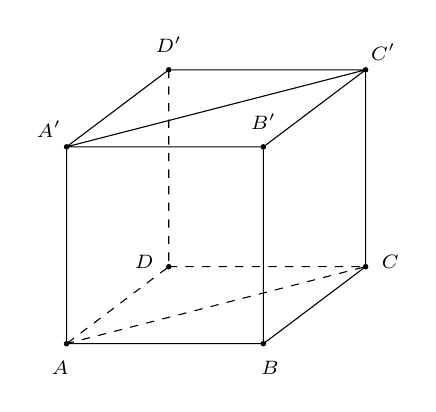
\begin{tikzpicture}[declare function={r=2.5;},font=\scriptsize]
			\path (0:0) coordinate (A)
			(0:r) coordinate (B)
			++(37:{0.65*r}) coordinate (C)
			++(180:r) coordinate (D)
			\foreach \x in {A,B,C,D}{(\x)++(90:r) coordinate (\x_1)};
			\draw[dashed] (D_1)--(D)--(A) (D)--(C)--(A);
			\draw (A)--(B)--(C) (A)--(A_1) (B)--(B_1) (C)--(C_1)(A_1)--(B_1)--(C_1)--(D_1)--cycle (A_1)--(C_1);
			\foreach \x/\goc/\t in {A/255/A, B/-75/B, C/10/C, D/170/D, A_1/135/A', B_1/90/B',
				C_1/45/C', D_1/90/D'}{
				\fill (\x) circle (1pt) node[shift={(\goc:9pt)}]{$\t$};
			}
	\end{tikzpicture}}
	\loigiai{
		Vì $ACC'A'$ là hình vuông có diện tích bằng $18$ nên độ dài cạnh của hình vuông là
		\[AA' = AC = \sqrt{18} = 3\sqrt{2}.\]
		Do lăng trụ $ABCD. A'B'C'D'$ là lăng trụ đều nên đáy $ABCD$ là hình vuông và chiều cao của lăng trụ là $h = AA' = 3\sqrt{2}$.\\
		Gọi $a$ là độ dài cạnh của đáy $ABCD$. \\
		Vì đáy là hình vuông nên đường chéo $AC = a\sqrt{2}$.\\
		Theo giả thiết ta có $AC = 3\sqrt{2}\Leftrightarrow a\sqrt{2} = 3\sqrt{2} \Leftrightarrow a = 3$.\\
		Diện tích đáy $ABCD$ là $S_{ABCD} = a^2 = 3^2 = 9$.\\
		Thể tích khối lăng trụ đều là $V = S_{ABCD} \cdot h = 9 \cdot 3\sqrt{2} = 27\sqrt{2}$.
	}
\end{ex}
\cauds
\begin{ex}%[2D1H2-1]%[Dương Công Tạo]
	Trong mặt phẳng toạ độ $Oxy$, cho hàm số $y = f(x) = x^3 - 3x^2 + 4$ có đồ thị $(C)$.
	\choiceTF
	{\True $f'(x) = 3x^2 - 6x$}
	{\True $f(x)$ nghịch biến trên đoạn $[0;2]$}
	{$\min\limits_{[-2;3]} f(x) = 0$}
	{\True $(C)$ có hai điểm cực trị cách nhau một khoảng bằng $2\sqrt{5}$}
	\loigiai{
		Xét hàm số $y = f(x) = x^3 - 3x^2 + 4$ trên khoảng $(\infty;+\infty)$.
		\begin{itemchoice}
			\itemch Ta có $f'(x) = 3x^2 - 6x$.
			\itemch Ta có $f'(x) = 3x^2 - 6x$; $f'(x)0 \Leftrightarrow 3x^2 - 6x=0\Leftrightarrow\hoac{&x=0\\x=2.}$\\
			Bảng biến thiên
			\begin{center}
				
\begin{tikzpicture}[>=stealth]
					\tkzTabInit[nocadre=false,lgt=1.5,espcl=2,deltacl=0.6]{$x$/.7 ,$f'(x)$/.7,$f(x)$/2}
					{$-\infty$ , $0$ , $2$ , $+\infty$}
					\tkzTabLine{ , + , $0$ , - , $0$ , + , }
					\tkzTabVar{-/$-\infty$ , +/$4$ , -/$0$ , +/$+\infty$}
				\end{tikzpicture}
			\end{center}
			Vì hàm số xác định trên $\mathbb{R}$ nên nó liên tục tại các điểm $x=0$ và $x=2$. \\
			Kết hợp với bảng biến thiên, ta thấy $f(x)$ nghịch biến trên đoạn $[0;2]$.
			\itemch Hàm số đã cho xác định và liên tục trên $[-2;3]$.\\
			Ta có $f'(x) = 3x^2 - 6x$; $f'(x)=0 \Leftrightarrow 3x^2 - 6x=0\Leftrightarrow\hoac{&x=0\in[-2;3]\\&x=2\in[-2;3].}$\\
			Mà $f(-2)=16$; $f(0)=4$; $f(2)=0$; $f(3)=4$ nên $\min\limits_{[-2;3]} f(x)=f(-2)= -16$.
			\itemch Gọi $A(0;4)$ và $B(2;0)$ là hai điểm cực trị của đồ thị $(C)$.\\
			Ta có $AB=\sqrt{(2-0)^2+(0-4)^2}=2\sqrt{5}$.
		\end{itemchoice}
	}
\end{ex}

\begin{ex}%[TDMZZ25]%[Hà Văn Hảo]%[2D4V2-6]
	Một vật tham gia chuyển động thẳng bắt đầu từ A đến $B$ và dừng lại tại $B$, với biểu thức vận tốc là $v(t)=at^2+bt$ m/s, ($a,b \in \mathbb{R}$, $a<0$), trong đó $t$ là thời gian (tính bằng giây). Biết rằng $AB = 480$ m và tổng thời gian vật đi từ $A$ đến $B$ là $36$ giây.
	\choiceTF
	{\True $36a+b=0$}
	{\True Vật chuyển động nhanh nhất ở thời điểm $t=18$ giây}
	{\True $a=-\dfrac{5}{81}$}
	{\True Tốc độ lớn nhất của vật đạt $20$ m/s}
	\loigiai{
		\begin{itemchoice}
			\itemch Vật dừng lại tại $B$ sau $36$ giây, tức là tại $t=36$ thì $v(36)=0$.\\
			Ta có $a(36)^2 + b(36) = 0 \Leftrightarrow 36a + b = 0$.
			\itemch Hàm vận tốc $v(t)=at^2+bt$ là một hàm số bậc hai có đồ thị là một parabol quay bề lõm xuống dưới ($a<0$).\\
			Vận tốc đạt giá trị lớn nhất tại đỉnh của parabol
			$t = -\dfrac{b}{2a} = -\dfrac{-36a}{2a} = 18$ giây.
			\itemch Quãng đường vật đi từ $A$ đến $B$ là
			\allowdisplaybreaks
			\begin{eqnarray*}
				AB &=& \displaystyle\int\limits_0^{36} v(t)\,\mathrm{d}t = 480\\
				&\Leftrightarrow& \displaystyle\int\limits_0^{36} (at^2 - 36at)\,\mathrm{d}t = 480 \\
				&\Leftrightarrow& \left.\left( \dfrac{at^3}{3} - 18at^2 \right)\right|_0^{36} = 480\\
				&\Leftrightarrow& a \cdot \dfrac{36^3}{3} - 18a \cdot 36^2 = 480 \Leftrightarrow 15\,552a - 23\,328a = 480\\
				&\Leftrightarrow& -7\,776a = 480 \\
				&\Leftrightarrow& a = -\dfrac{5}{81}
			\end{eqnarray*}
			\itemch Với $a = -\dfrac{5}{81}$ và $b = -36a = \dfrac{180}{81} = \dfrac{20}{9}$.\\
			Vận tốc lớn nhất tại $t=18$ là $v(18) = -\dfrac{5}{81} \cdot 18^2 + \dfrac{20}{9} \cdot 18 = 20$ m/s.
		\end{itemchoice}
	}
\end{ex}

\begin{ex}%[2H5V2-8]%[TDMZZ25]%[Vũ Hồng Toàn]
	Trong không gian $Oxyz$ có đơn vị dài mỗi trục là mét, một cabin trong hệ thống cáp treo xuất phát từ điểm $A(-2;3;8)$ chuyển động thẳng đều theo hướng vectơ $\overrightarrow{u} = (4;3;-1)$ với tốc độ $3$\,m/s. Sau $5$ giây kể từ lúc xuất phát, cabin đến điểm $B(a;b;c)$.
	\choiceTF
	{\True Hai vectơ $\overrightarrow{AB}$ và $\overrightarrow{u}$ cùng hướng với nhau}
	{\True Phương trình tham số đường thẳng $AB$ là $\heva{&x = -2 + 4t \\& y = 3 + 3t \\& z = 8 - t}, t \in \mathbb{R}$}
	{$AB = 5\sqrt{26}\text{ m}$}
	{$a + 2b + c = 32$}
	\loigiai{
		\begin{itemchoice}
			\itemch Cabin chuyển động thẳng đều từ $A(-2;3;8)$ theo hướng của vectơ $\overrightarrow{u} = (4;3;-1)$ nên vectơ chỉ phương của đường thẳng $AB$ là $\overrightarrow{u} = (4;3;-1)$.\\ Do đó, hai vectơ $\overrightarrow{AB}$ và $\overrightarrow{u}$ cùng hướng với nhau.
			\itemch Đường thẳng $AB$ đi qua $A(-2;3;8)$ và có vectơ chỉ phương $\overrightarrow{u} = (4;3;-1)$ nên có phương trình tham số là
			$\heva{&x = -2 + 4t \\& y = 3 + 3t \\& z = 8 - t}, t \in \mathbb{R}.$
			\itemch Tốc độ của cabin là $v = 3$\,m/s.\\ Sau $5$ giây kể từ lúc xuất phát, quãng đường cabin đi được là $AB = v \cdot t = 3 \cdot 5 = 15$\,m.
			\itemch Ta có $\left|\overrightarrow{u}\right| = \sqrt{4^2 + 3^2 + (-1)^2} = \sqrt{26}$.\\
			Vì cabin chuyển động cùng hướng với $\overrightarrow{u}$ nên \[\overrightarrow{AB} = \dfrac{AB}{\left|\overrightarrow{u}\right|} \overrightarrow{u} = \dfrac{15}{\sqrt{26}}\cdot (4; 3; -1) = \left(\dfrac{60}{\sqrt{26}}; \dfrac{45}{\sqrt{26}}; -\dfrac{15}{\sqrt{26}}\right).\]
			Tọa độ điểm $B(a; b; c)$ là $\heva{&a = -2 + \dfrac{60}{\sqrt{26}} \\& b = 3 + \dfrac{45}{\sqrt{26}} \\& c = 8 - \dfrac{15}{\sqrt{26}}.}$\\
			Suy ra $a + 2b + c = -2 + \dfrac{60}{\sqrt{26}} + 2\cdot\left(3 + \dfrac{45}{\sqrt{26}}\right) + 8 - \dfrac{15}{\sqrt{26}} \approx 38{,}47$.
		\end{itemchoice}
	}
\end{ex}

\begin{ex}%[2D6V1-2]%[TDMZZ25]%[Văn Minh Thoại]
	Tiến hành gieo ngẫu nhiên một con xúc xắc cân đối đồng chất hai lần liên tiếp. Gọi $A$ là biến cố lần thứ nhất xuất hiện số chấm lớn hơn $3$, $B$ là biến cố tổng số chấm ở hai lần gieo nhỏ hơn $7$.
	\choiceTF
	{\True $\mathrm{P}(A)=\dfrac{1}{2}$}
	{\True $\mathrm{P}(B)=\dfrac{5}{12}$}
	{\True $\mathrm{P}(AB)=\dfrac{1}{12}$}
	{\True $\mathrm{P}(A \mid B)+P(B \mid A)=\dfrac{11}{30}$}
	\loigiai{
		Gọi $i$, $j$ lần lượt là số chấm xuất hiện ở lần gieo thứ nhất và thứ hai ($i$, $j \in \{1; 2; 3; 4; 5; 6\}$).\\
		Không gian mẫu $\Omega = \{(i; j) \mid 1 \le i, j \le 6\}$. \\
		Số phần tử của không gian mẫu là $n(\Omega) = 6 \cdot 6 = 36$.\\
		Ta có thể minh họa không gian mẫu và các biến cố qua hệ trục tọa độ như sau (mỗi điểm lưới tương ứng với một kết quả)
		\begin{center}
			\begin{tikzpicture}[scale=0.8,>=stealth]
				\draw[->,thick] (0,0) -- (7.5,0) node[below] {Lần $1$($i$)};
				\draw[->,thick] (0,0) -- (0,7.5) node[left] {Lần $2$($j$)};
				\foreach \x in {1,...,6}{
					\draw (\x,0.1) -- (\x,-0.1) node[below] {\small $\x$};
					\draw (0.1,\x) -- (-0.1,\x) node[left] {\small $\x$};
				}
				% Grid points
				\foreach \i in {1,...,6}{
					\foreach \j in {1,...,6}{
						\fill[gray!40] (\i,\j) circle (3pt);
					}
				}
				% Biến cố A: i > 3
				\fill[blue,opacity=0.1,rounded corners=5pt] (3.5,0.5) rectangle (6.5,6.5);
				\draw[blue,thick,rounded corners=5pt] (3.5,0.5) rectangle (6.5,6.5);
				\node[blue,above] at (5,6.5) {\textbf{Biến cố $A$}};
				% Biến cố B: i + j < 7
				\draw[red,thick,dashed] (0.5,6.5) -- (6.5,0.5);
				% Điểm thuộc A giao B
				\foreach \i/\j in {4/1,4/2,5/1}{
					\fill[green!70!black] (\i,\j) circle (4pt);
					\draw[green!70!black,thick] (\i,\j) circle (6pt); }
				% Legend
				\begin{scope}[shift={(8,4.5)}]
					\fill[gray!40] (0,1) circle (3pt); \node[right] at (0.2,1) {Điểm thuộc $\Omega$};
					\fill[blue,opacity=0.3] (-0.1,-0.1) rectangle (0.1,0.1); \node[right] at (0.2,0) {Biến cố $A$($i>3$)};
					\draw[red,thick,dashed] (-0.2,-1) -- (0.2,-1); \node[right] at (0.2,-1) {Tổng số chấm bằng $7$($i+j=7$)};
					\fill[green!70!black] (0,-2) circle (4pt);
					\draw[green!70!black,thick] (0,-2) circle (6pt); \node[right] at (0.2,-2) {Biến cố $A \cap B$};
				\end{scope}
			\end{tikzpicture}
		\end{center}
		\begin{itemchoice}
			\itemch Biến cố $A\colon$\lq\lq Lần thứ nhất xuất hiện số chấm lớn hơn $3$\rq\rq.\\
			Ta có $i \in \{4; 5; 6\}$ và $j \in \{1; 2; 3; 4; 5; 6\}$.\\
			Số phần tử của $A$ là $n(A) = 3\cdot6 = 18$.\\
			Suy ra $\mathrm{P}(A)=\dfrac{18}{36}=\dfrac{1}{2}$.
			\itemch Biến cố $B\colon$\lq\lq Tổng số chấm ở hai lần gieo nhỏ hơn $7$\rq\rq.\\
			Các kết quả thuận lợi cho $B$ là $(i; j)$ sao cho $i + j < 7$:
			\begin{itemize}
				\item $i=1 \Rightarrow j \in \{1; 2; 3; 4; 5\}$ (có $5$ kết quả).
				\item $i=2 \Rightarrow j \in \{1; 2; 3; 4\}$ (có $4$ kết quả).
				\item $i=3 \Rightarrow j \in \{1; 2; 3\}$ (có $3$ kết quả).
				\item $i=4 \Rightarrow j \in \{1; 2\}$ (có $2$ kết quả).
				\item $i=5 \Rightarrow j \in \{1\}$ (có $1$ kết quả).
			\end{itemize}
			Số phần tử của $B$ là $n(B) = 5+4+3+2+1 = 15$.\\
			Suy ra $\mathrm{P}(B)=\dfrac{15}{36}=\dfrac{5}{12}$.
			
			\itemch Biến cố $A \cap B$ (hay $AB$)$\colon$\lq\lq Lần thứ nhất lớn hơn $3$ và tổng hai lần nhỏ hơn $7$\rq\rq.\\
			Ta có điều kiện $\heva{&i \in \{4; 5; 6\} \\ &i+j < 7} \Rightarrow \heva{&i \in \{4; 5; 6\} \\ &j < 7-i}$.
			\begin{itemize}
				\item $i=4 \Rightarrow j < 3 \Rightarrow j \in \{1; 2\}$.
				\item $i=5 \Rightarrow j < 2 \Rightarrow j \in \{1\}$.
				\item $i=6 \Rightarrow j < 1$ (không có $j$ thỏa mãn).
			\end{itemize}
			Tập hợp $A \cap B = \{(4; 1); (4; 2); (5; 1)\}$. \\
			Số phần tử là $n(AB) = 3$.\\
			Suy ra $\mathrm{P}(AB) = \dfrac{3}{36} = \dfrac{1}{12}$.
			\itemch Ta có
			\begin{itemize}
				\item $\mathrm{P}(A \mid B) = \dfrac{\mathrm{P}(AB)}{\mathrm{P}(B)} = \dfrac{\dfrac{1}{12}}{\dfrac{5}{12}}=\dfrac{1}{5}$;
				\item $\mathrm{P}(B \mid A)=\dfrac{\mathrm{P}(AB)}{\mathrm{P}(A)}=\dfrac{\dfrac{1}{12}}{\dfrac{1}{2}}=\dfrac{2}{12}=\dfrac{1}{6}$.
			\end{itemize}
			Suy ra $\mathrm{P}(A \mid B) + \mathrm{P}(B \mid A)=\dfrac{1}{5}+\dfrac{1}{6}=\dfrac{11}{30}$.
		\end{itemchoice}
	}
\end{ex}
\caukq
\begin{ex}%[2D4H1-6]%[TDMZZ25]%[Lê Hồ Quang Minh]
	Cho hàm chi phí biên $f(x) = 0{,}06x^2 - 3x + 30$ nghìn đồng/sản phẩm. Biết chi phí cố định là $10$ triệu đồng. Hãy tính theo đơn vị triệu đồng tổng chi phí khi sản xuất $80$ sản phẩm \textit{(làm tròn kết quả đến hàng đơn vị)}?
	\par\shortans[oly]{13}
	\loigiai{
		Tổng chi phí để sản xuất $x$ sản phẩm là
		\[C(x) = \displaystyle\int (0{,}06x^2 - 3x + 30) \, \mathrm{\,d}x = 0{,}02x^3 - 1{,}5x^2 + 30x + C \quad (\text{nghìn đồng}),\]
		Theo giả thiết ta có
		\[C(0) = 10\,000 \Leftrightarrow C = 10\,000.\]
		Suy ra hàm tổng chi phí là
		\[C(x) = 0{,}02x^3 - 1{,}5x^2 + 30x + 10\,000.\]
		Suy ra tổng chi phí khi sản xuất $80$ sản phẩm là $C(80) = 13\,040$ (nghìn đồng).\\
		Vậy tổng chi phí theo đơn vị triệu đồng $\approx 13$ triệu đồng.
	}
\end{ex}
\begin{ex}
	content
\end{ex}
\begin{ex}%[2H2V2-6]%[TDMZZ25-19-TLN]%[Đỗ Đường Hiếu]
	Trong không gian $Oxyz$ có đơn vị dài trên mỗi trục là mét, mặt đất là mặt phẳng $(Oxy)$. Từ gốc tọa độ $O$, một vật thực hiện chuyển động ném xiên với vận tốc là $\overrightarrow{v}=(18;18;24)$ với đơn vị m/s. Biết rằng vị trí $M$ của vật sau $t$ giây được xác định bởi biểu thức $\overrightarrow{OM} = t\overrightarrow{v} + \dfrac{1}{2}t^2\overrightarrow{g}$, với $\overrightarrow{g}=(0;0;-10)$. Hỏi khi vật ở độ cao cực đại thì vật cách gốc tọa độ $O$ bao nhiêu centimet (\textit{không làm tròn ở các phép tính trung gian và làm tròn kết quả đến hàng đơn vị})?
	\par\shortans{6754}
	\loigiai{
		Vị trí của vật tại thời điểm $t$ là
		$$\overrightarrow{OM} = t(18; 18; 24) + \dfrac{1}{2}t^2(0; 0; -10) = (18t; 18t; 24t - 5t^2).$$
		Tọa độ của vật là $M\left(18t; 18t; 24t - 5t^2\right)$.\\
		Độ cao của vật là $z(t) = 24t - 5t^2$.\\
		Vật đạt độ cao cực đại khi $z'(t) = 24 - 10t = 0 \Leftrightarrow t = 2{,}4$ (giây).\\
		Khi đó, vị trí của vật là $M\left(43{,}2;43{,}2;28{,}8\right)$.\\
		Ta có $OM = \sqrt{(43{,}2)^2 + (43{,}2)^2 + (28{,}8)^2} \approx 67{,}542$ (mét).\\
		Đổi sang centimet: $67{,}542 \times 100 = 6754{,}2$ cm.\\
		Làm tròn đến hàng đơn vị ta được $6754$ cm.
	}
\end{ex}

\begin{ex}%[2D4C3-1]%[TDMZZ25]%[Nguyễn Đức Tuấn Anh]
	\immini[thm]{
		Trên mặt phẳng tọa độ $Oxy$, cho hai hình tròn và parabol $(P)\colon y=x^2$ như hình vẽ. Hình tròn nhỏ có tâm $(0;10)$, hai hình tròn này tiếp xúc với nhau và tiếp xúc với $(P)$. Hãy tính diện tích phần tô màu (\textit{làm tròn kết quả đến hàng phần mười})?
	}{
		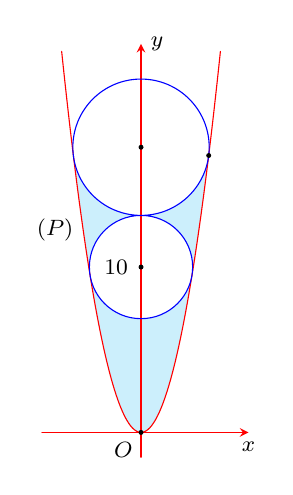
\begin{tikzpicture}[scale=.6, font=\footnotesize, line join=round, line cap=round, >=stealth]
			\begin{scope}[x=0.35cm, y=0.35cm]
				\pgfmathsetmacro{\Rone}{sqrt(9.75)}
				\pgfmathsetmacro{\Rtwo}{\Rone + 1}
				\pgfmathsetmacro{\ytwo}{11 + 2*\Rone}
				\pgfmathsetmacro{\yPtwo}{\ytwo - 0.5}
				\pgfmathsetmacro{\xPtwo}{sqrt(\yPtwo)}
				\pgfmathsetmacro{\thetaTwo}{asin(-0.5 / \Rtwo)}
				
				\path (0,0) coordinate (O) 
				(0,10) coordinate (I1) 
				(0,\ytwo) coordinate (I2) 
				(\xPtwo,\yPtwo) coordinate (P2);
				
				\fill[cyan!20] plot[domain=-\xPtwo:\xPtwo, samples=100] (\x, {\x*\x}) arc (\thetaTwo:-180-\thetaTwo:\Rtwo) -- cycle;
				\fill[white] (I1) circle (\Rone);
				
				\draw[->, red] (-6,0) -- (6.5,0);
				\draw[->, red] (0,-1.5) -- (0,23.5);
				\draw[red] plot[domain=-4.8:4.8, samples=100] (\x, {\x*\x});
				
				\draw[blue] (I1) circle (\Rone) (I2) circle (\Rtwo);
				
				\fill (O) circle (1.5pt) (I1) circle (1.5pt) (I2) circle (1.5pt) (P2) circle (1.5pt);
				
				\path (6.5,0) node[below] {$x$}
				(0,23.5) node[right] {$y$}
				(-3.5,12.25) node[left] {$(P)$};
				
				\foreach \p/\ang/\d/\lbl in {O/-135/1.5/O, I1/180/1.5/10}
				\path (\p) ++(\ang:\d) node {$\lbl$};
			\end{scope}
		\end{tikzpicture}
	}
	\par\shortans{38{,}1}
	\loigiai{
		Gọi $(C_1)$ là hình tròn nhỏ tâm $I_1(0;10)$, bán kính $R_1$.\\
		Phương trình đường tròn $(C_1)$ là $x^2 + (y-10)^2 = R_1^2$.\\
		Vì $(C_1)$ tiếp xúc với parabol $(P)\colon y = x^2$ nên hệ phương trình $\heva{&y=x^2\\&x^2+(y-10)^2=R_1^2}$ có nghiệm duy nhất ($y \ge 0$).\\
		Thay $x^2=y$ ta được $y^2 - 19y + 100 - R_1^2 = 0$.\\
		Điều kiện để phương trình có nghiệm kép là
		\[\Delta_1 = 19^2 - 4\left(100 - R_1^2\right) = 0 \Leftrightarrow 4R_1^2 = 39 \Rightarrow R_1 = \dfrac{\sqrt{39}}{2}.\]
		Gọi $(C_2)$ là hình tròn lớn tâm $I_2(0;b)$, bán kính $R_2$ (với $b > 10$, $R_2 > 0$).\\
		Phương trình của $(C_2)$ là $x^2 + (y-b)^2 = R_2^2$.\\
		Vì $(C_2)$ tiếp xúc ngoài với $(C_1)$ và có tâm nằm trên trục $Oy$ nên
		\[b - 10 = R_1 + R_2 \Leftrightarrow b = 10 + R_1 + R_2.\]
		Vì $(C_2)$ tiếp xúc với $(P)$ nên tương tự, phương trình hoành độ giao điểm $y^2 + (1-2b)y + b^2 - R_2^2 = 0$ có nghiệm kép.\\
		Điều kiện là $\Delta_2 = (1-2b)^2 - 4(b^2 - R_2^2) = 0 \Leftrightarrow 4R_2^2 = 4b - 1$.\\
		Thay $b = 10 + R_1 + R_2$ vào ta được
		\[4R_2^2 = 40 + 4R_1 + 4R_2 - 1 = 39 + 4R_1 + 4R_2.\]
		Do $39 = 4R_1^2$ nên ta có phương trình
		\[4R_2^2 - 4R_2 = 4R_1^2 + 4R_1 \Leftrightarrow R_2^2 - R_1^2 - (R_2 + R_1) = 0 \Leftrightarrow (R_2 + R_1)(R_2 - R_1 - 1) = 0.\]
		Vì $R_2 + R_1 > 0$, suy ra $R_2 - R_1 - 1 = 0 \Rightarrow R_2 = R_1 + 1 = \dfrac{\sqrt{39}}{2} + 1$.\\
		Tọa độ $y$ của tiếp điểm giữa $(C_2)$ và $(P)$ là nghiệm kép $y_2 = \dfrac{2b-1}{2} = b - 0{,}5$.\\
		Với $b = 10 + R_1 + R_2 = 11 + 2R_1 = 11 + \sqrt{39}$, ta tính được $y_2 = 10{,}5 + \sqrt{39}$.\\
		Diện tích phần tô màu $S$ bằng diện tích hình phẳng giới hạn bởi parabol $(P)$ và đường thẳng $y=y_2$, bỏ đi diện tích hình tròn $(C_1)$ và diện tích hình viên phân của $(C_2)$ nằm dưới đường thẳng $y=y_2$.\\
		Ta có $S = S_P - S_1 - S_q$, trong đó
		\begin{itemize}
			\item $S_P$ là diện tích hình phẳng giới hạn bởi $(P)$ và đường thẳng $y=y_2$
			\[S_P = \displaystyle\int\limits_{-\sqrt{y_2}}^{\sqrt{y_2}} \left(y_2 - x^2\right) \mathrm{\,d}x = \dfrac{4}{3}y_2\sqrt{y_2} \approx 91{,}36.\]
			\item $S_1$ là diện tích hình tròn $(C_1)$
			\[S_1 = \pi R_1^2 = \dfrac{39\pi}{4} \approx 30{,}63.\]
			\item $S_q$ là diện tích hình viên phân của $(C_2)$ giới hạn bởi cung nhỏ và dây cung thuộc đường thẳng $y=y_2$.\\
			Khoảng cách từ tâm $I_2(0;b)$ đến đường thẳng $y=y_2$ là $d = b - y_2 = 0{,}5$.\\
			Gọi $\alpha$ là góc ở tâm chắn cung viên phân này, ta có $\cos \dfrac{\alpha}{2} = \dfrac{d}{R_2} = \dfrac{0{,}5}{R_2}$. \\
			Diện tích viên phân là
			\[S_q = R_2^2 \arccos \left(\dfrac{0{,}5}{R_2}\right) - d\sqrt{R_2^2 - d^2} = R_2^2 \arccos \left(\dfrac{1}{2R_2}\right) - 0{,}5\sqrt{y_2} \approx 22{,}58.\]
		\end{itemize}
		Vậy diện tích phần tô màu là
		\[S = S_P - S_1 - S_q \approx 91{,}36 - 30{,}63 - 22{,}58 = 38{,}1.\]
	}
\end{ex}
\begin{ex}
	content
\end{ex}
\begin{ex}%[0D0C2-3]%[TDM42]%[Nguyễn Văn Sang]
	Có $24$ chiếc bàn học được chia thành $3$ dãy $8$ hàng, mỗi hàng có ba chiếc bàn như hình vẽ. Thầy chủ nhiệm xếp ngẫu nhiên $24$ em học sinh của lớp vào $24$ chiếc bàn này sao cho mỗi em ngồi một bàn. Biết rằng lớp có $5$ học sinh giỏi xuất sắc, $3$ em học sinh giỏi, $2$ em học sinh khá và còn lại là trung bình. Gọi $p$ là xác suất để xếp được mỗi hàng không có nhiều hơn một học sinh cùng xuất sắc hoặc cùng giỏi hoặc cùng khá. Hãy tính $10000p$ \textit{(làm tròn kết quả đến hàng đơn vị)}?
	\begin{center}
		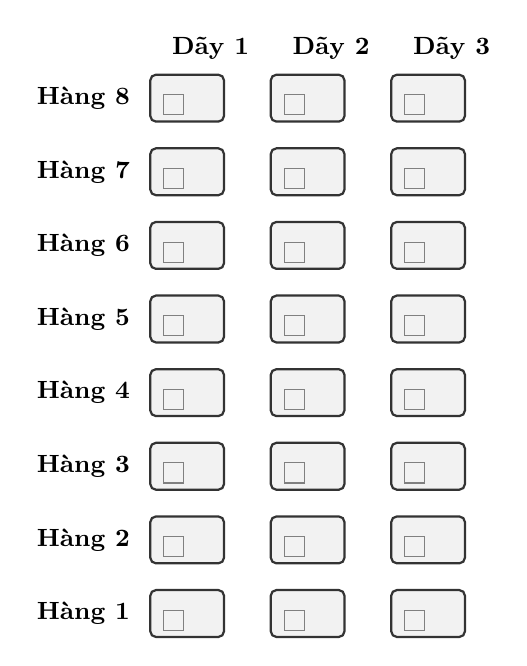
\begin{tikzpicture}[scale=0.85, >=stealth]
			% Đã đổi toàn bộ hình vẽ sang tone Trắng - Đen - Xám chuẩn đề thi in giấy
			\foreach \r in {1,...,8} {
				\foreach \c in {1,...,3} {
					\draw[thick, fill=gray!10, draw=black!80, rounded corners=2pt] (\c*1.8-0.6, \r*1.1-0.4) rectangle ++(1.1,0.7);
					\draw[thin, draw=black!50] (\c*1.8-0.4, \r*1.1-0.3) rectangle ++(0.3,0.3);
				}
				\node[font=\small\bfseries] at (0.2, \r*1.1-0.05) {Hàng \r};
			}
			\node[font=\bfseries\small] at (2.1, 9.5) {Dãy 1};
			\node[font=\bfseries\small] at (3.9, 9.5) {Dãy 2};
			\node[font=\bfseries\small] at (5.7, 9.5) {Dãy 3};
		\end{tikzpicture}
	\end{center}
	\par\shortans[0]{2239}
	\loigiai{
		\textbf{Bước 1: Tính số phần tử của không gian mẫu}\\
		Xếp ngẫu nhiên $24$ học sinh vào $24$ chiếc bàn phân biệt:
		$$n(\Omega) = 24! \text{ (cách)}$$
		\textbf{Bước 2: Phân tích bài toán và Phương pháp giải}\\
		Lớp có $5$ bạn Xuất sắc (XS), $3$ bạn Giỏi (G), $2$ bạn Khá (K) và $14$ bạn Trung bình (TB).
		Điều kiện bài toán: \textit{Mỗi hàng ngang không có quá $1$ XS, không quá $1$ G, không quá $1$ K}. (Lưu ý: Các nhóm này được phép ngồi chung hàng với nhau, miễn là không trùng loại).\\
		Để tránh sai sót, ta chia quá trình sắp xếp thành 2 công đoạn
		\begin{itemize}
			\item \textbf{Công đoạn 1:} Thiết kế sơ đồ chỗ ngồi (Lần lượt chọn và "dán nhãn" ghế cho nhóm XS, rồi đến G, rồi đến K).
			\item \textbf{Công đoạn 2:} Mời từng học sinh cụ thể vào đúng chiếc ghế đã dán nhãn.
		\end{itemize}
		\textbf{Bước 3: Thiết kế sơ đồ chỗ ngồi (Công đoạn 1)}\\
		\textbf{1. Chọn ghế cho nhóm Xuất sắc (XS):}
		\begin{itemize}
			\item Chọn $5$ hàng (trong $8$ hàng), mỗi hàng chọn $1$ ghế: Có $\mathrm{C}_8^5 \cdot 3^5 = \mathbf{13608} \text{ (cách)}$.
			\item \textit{Tình trạng lớp lúc này:} Gồm \textbf{$5$ hàng} bị chiếm $1$ chỗ (còn $2$ trống) và \textbf{$3$ hàng} chưa ai ngồi (còn $3$ trống).
		\end{itemize}
		\textbf{2. Chọn ghế cho nhóm Giỏi (G) và Khá (K) bằng Bảng:}
		Nhóm G ($3$ bạn) chọn ghế ở $3$ hàng khác nhau. Ta xét số lượng hàng mà nhóm G "ngồi chung" với nhóm XS, từ đó suy ra chỗ trống còn lại cho nhóm K ($2$ bạn):
		\begin{center}
			\renewcommand{\arraystretch}{1.5}
			\begin{tabular}{|p{0.3\linewidth}|p{0.3\linewidth}|p{0.32\linewidth}|}
				\hline
				\centering\textbf{Trường hợp nhóm G} & \centering\textbf{Số cách cho nhóm G} & \multicolumn{1}{c|}{\textbf{Cấu trúc ghế trống để xếp Khá}} \\ \hline
				\textbf{TH0: Ngồi chung XS $0$ hàng} \newline
				\textit{(G chọn $0$ hàng đang có 2 trống \newline \& $3$ hàng đang có 3 trống)}
				& Chọn chung: $\mathrm{C}_5^0 \cdot 2^0 = 1$ \newline
				Chọn riêng: $\mathrm{C}_3^3 \cdot 3^3 = 27$ \newline
				$\Rightarrow 1 \times 27 = \mathbf{27}$ (cách)
				& $\bullet$ \textbf{8 hàng:} còn $2$ trống. \newline
				$\Rightarrow$ Cách xếp 2 K: \textbf{112 cách (*)} \\ \hline
				\textbf{TH1: Ngồi chung XS $1$ hàng} \newline
				\textit{(G chọn $1$ hàng đang có 2 trống \newline \& $2$ hàng đang có 3 trống)}
				& Chọn chung: $\mathrm{C}_5^1 \cdot 2^1 = 10$ \newline
				Chọn riêng: $\mathrm{C}_3^2 \cdot 3^2 = 27$ \newline
				$\Rightarrow 10 \times 27 = \mathbf{270}$ (cách)
				& $\bullet$ \textbf{1 hàng:} còn $1$ trống. \newline
				$\bullet$ \textbf{6 hàng:} còn $2$ trống. \newline
				$\bullet$ \textbf{1 hàng:} còn $3$ trống. \newline
				$\Rightarrow$ Cách xếp 2 K: \textbf{111 cách (*)} \\ \hline
				\textbf{TH2: Ngồi chung XS $2$ hàng} \newline
				\textit{(G chọn $2$ hàng đang có 2 trống \newline \& $1$ hàng đang có 3 trống)}
				& Chọn chung: $\mathrm{C}_5^2 \cdot 2^2 = 40$ \newline
				Chọn riêng: $\mathrm{C}_3^1 \cdot 3^1 = 9$ \newline
				$\Rightarrow 40 \times 9 = \mathbf{360}$ (cách)
				& $\bullet$ \textbf{2 hàng:} còn $1$ trống. \newline
				$\bullet$ \textbf{4 hàng:} còn $2$ trống. \newline
				$\bullet$ \textbf{2 hàng:} còn $3$ trống. \newline
				$\Rightarrow$ Cách xếp 2 K: \textbf{110 cách (*)} \\ \hline
				
				\textbf{TH3: Ngồi chung XS $3$ hàng} \newline
				\textit{(G chọn $3$ hàng đang có 2 trống \newline \& $0$ hàng đang có 3 trống)}
				& Chọn chung: $\mathrm{C}_5^3 \cdot 2^3 = 80$ \newline
				Chọn riêng: $1$ \newline
				$\Rightarrow 80 \times 1 = \mathbf{80}$ (cách)
				& $\bullet$ \textbf{3 hàng:} còn $1$ trống. \newline
				$\bullet$ \textbf{2 hàng:} còn $2$ trống. \newline
				$\bullet$ \textbf{3 hàng:} còn $3$ trống. \newline
				$\Rightarrow$ Cách xếp 2 K: \textbf{109 cách (*)} \\ \hline
			\end{tabular}
		\end{center}
		\textit{(*) Tính toán số cách xếp chỗ cho nhóm Khá (chọn $2$ ghế ở $2$ hàng khác nhau):}
		\begin{itemize}
			\item \textbf{TH0:} Cả $2$ ghế vào $2$ hàng bất kỳ (mỗi hàng có 2 trống): $\mathrm{C}_8^2 \cdot 2^2 = \mathbf{112}$.
			\item \textbf{TH1:} Căn cứ vào số lượng hàng trống ở cột 3, ta có $$(\mathrm{C}_6^2 \cdot 2^2) + (\mathrm{C}_1^1 \cdot 1 \cdot \mathrm{C}_6^1 \cdot 2) + (\mathrm{C}_1^1 \cdot 1 \cdot \mathrm{C}_1^1 \cdot 3) + (\mathrm{C}_6^1 \cdot 2 \cdot \mathrm{C}_1^1 \cdot 3) = \mathbf{111}$$
			\item \textbf{TH2:} Căn cứ vào số lượng hàng trống ở cột 3, ta có $$(\mathrm{C}_2^2 \cdot 1^2) + (\mathrm{C}_4^2 \cdot 2^2) + (\mathrm{C}_2^2 \cdot 3^2) + (\mathrm{C}_2^1 \cdot 1 \cdot \mathrm{C}_4^1 \cdot 2) + (\mathrm{C}_2^1 \cdot 1 \cdot \mathrm{C}_2^1 \cdot 3) + (\mathrm{C}_4^1 \cdot 2 \cdot \mathrm{C}_2^1 \cdot 3) = \mathbf{110}$$
			\item \textbf{TH3:} Căn cứ vào số lượng hàng trống ở cột 3, ta có $$(\mathrm{C}_3^2 \cdot 1^2) + (\mathrm{C}_2^2 \cdot 2^2) + (\mathrm{C}_3^2 \cdot 3^2) + (\mathrm{C}_3^1 \cdot 1 \cdot \mathrm{C}_2^1 \cdot 2) + (\mathrm{C}_3^1 \cdot 1 \cdot \mathrm{C}_3^1 \cdot 3) + (\mathrm{C}_2^1 \cdot 2 \cdot \mathrm{C}_3^1 \cdot 3) = \mathbf{109}$$
		\end{itemize}
		
		Tổng số sơ đồ vị trí hợp lệ cho $3$ nhóm XS, G, K là
		$$m = 13608 \times \Big[ (27 \times 112) + (270 \times 111) + (360 \times 110) + (80 \times 109) \Big] = \mathbf{1.106.520.912} \text{ (sơ đồ)}.$$
		\textbf{Bước 4: Tính xác suất (Công đoạn 2)}\\
		Ứng với $1.106.520.912$ sơ đồ đã định sẵn, ta xếp học sinh vào lớp
		\begin{itemize}
			\item Hoán vị các em XS, G, K vào đúng ghế nhóm mình: $5! \cdot 3! \cdot 2!$ (cách).
			\item Hoán vị $14$ em Trung bình vào $14$ ghế trống còn lại: $14!$ (cách).
		\end{itemize}
		Xác suất cần tìm của bài toán là
		$$p = \dfrac{1.106.520.912 \times 5! \times 3! \times 2! \times 14!}{24!} \approx 0,22388$$
		Ta có $10000p = 2238,8$. Làm tròn đến hàng đơn vị, kết quả là $\boxed{2239}$.
	}
\end{ex}